\documentclass[]{article}
% bib use
\usepackage{cite}
% tabular eqn
\usepackage{amsmath, array}
% code listing
\usepackage{listings}
% images
\usepackage{graphicx} 
% lock images
\usepackage{float}
% colored syntax highlighting
\usepackage{xcolor}  
%captions in listings
\usepackage{caption}

%opening
\title{Principles of statistical inference project - Part 1}
\author{Carmel Gafa'}

\begin{document}

\maketitle

% style for all code snippets
\lstset{
	basicstyle=\ttfamily\footnotesize,  % Use Courier (monospace)
	numbers=left, numberstyle=\tiny, stepnumber=1, numbersep=5pt,
	breaklines=true, breakatwhitespace=true,
	frame=single, rulecolor=\color{gray}  % Single-line frame
}



\section{Question 1}


\textbf{Consider a random variable $X$ that follows an exponential distribution with scale parameter $\lambda$.}
\bigskip

The \textbf{Exponential Distribution} is a continuous probability distribution that represents the time intervals between consecutive events in a Poisson process, where events happen independently and at a constant average rate. It is defined by a single parameter, $\lambda$, referred to as the rate parameter.


\subsection{Give reference to a publication in which the exponential distribution has been used in practise.  
	Explain the context in which this distribution has been used in this publication.}

Mahmud et al. presented a study where they analyzed and estimated response times to questions on Twitter\cite{mahmud2013will}. The authors developed predictive models to estimate response wait times, exploring three different approaches:

\begin{itemize}
	\item Personalized wait time models: These models estimate the wait time for a specific user based on their individual history of response wait times. They assume each response event for a user occurs continuously and independently at a constant average rate, modelled by an exponential distribution. Each user's rate parameter $\lambda$ is estimated as the inverse of their average past response wait times.
	
	These models demonstrated a promising ability to estimate response times on Twitter. They generally outperformed generalized models and showed reasonable accuracy, especially for an hour or more time limits. The choice of cut-off probability (a threshold used to determine whether a user is considered sufficiently likely to respond to a question on Twitter within a given period) significantly influenced the precision and recall of the predictions.
	
	\item Generalized wait time models: Instead of individual models, a single model is built using the previous responses of all users in the dataset, again using the exponential distribution. The rate parameter $\lambda$ is estimated from the responses of all users. This model underperformed compared to the personalized models in estimating response times on Twitter.
	
	
	\item Time-sensitive wait time models: These models incorporate sensitivity to the time of day or day of the week when questions are sent for both generalized and personalized models by calculating the rate parameter based on responses to questions sent during a specific day or hour. Personalized time-sensitive models only considered users with at least five responses during the modelled time interval. Incorporating time sensitivity had a modest positive impact on the generalized models but did not consistently improve the performance of the personalized models.
\end{itemize}


\subsection{State the mean and the variance of $X$.}

As $X$ follows an exponential distribution with scale parameter, $X \sim Exp(X)$, the expected value or mean is:
\begin{equation}
	E[X] = \frac{1}{\lambda}
\end{equation}
and the variance is:
\begin{equation}
	Var(X) = \frac{1}{\lambda^2}
\end{equation}


\subsection{ Derive the moment estimator of $\lambda$.}

The p.d.f. for an exponential distribution is:

\begin{equation}
	f(x)=\lambda e^{- \lambda x} \space,x \leq 0, \space \lambda > 0
\end{equation}


\noindent The first moment, or expected value:

\begin{flalign*}
E[X] &= \int_{0}^{\infty} x\space f(x) dx \\
		&= \int_{0}^{\infty} x \lambda e^{- \lambda x} dx \\
		&= \lambda \int_{0}^{\infty} x e^{- \lambda x}
\end{flalign*}

\noindent Integrating by parts, we let:

\begin{tabular}{ll}
$u = x$ 									& $du = (1) dx$ \\
$v = -\frac{e^{- \lambda x}}{\lambda}$	& $dv =  e^{- \lambda x} dx$
\end{tabular}

\bigskip
\noindent As $\int udv = uv -\int v du$:

\begin{flalign*}
E[X]	&= \lambda\left( \left[ - \frac{ x e^{- \lambda x}}{\lambda} \right]_0^\infty - \int_{0}^{\infty} -\frac{e^{- \lambda x}}{\lambda} (1) dx \right)\\
		&=   \left[ - x e^{- \lambda x}\right]_0^\infty + \int_{0}^{\infty} -e^{- \lambda x}dx
\end{flalign*}


\noindent Let us consider $\left[  x e^{- \lambda x}\right]_0^\infty$:
\begin{itemize}
	\item $- x e^{- \lambda x} = 0$, when $x=0$
	\item $\displaystyle \lim_{x \to \infty}  x e^{- \lambda x} = 0$, as exponential decay dominates polynomial growth
\end{itemize}

\noindent So the first term is removed;

\begin{flalign*}
	E[X] &=\int_{0}^{\infty} -e^{- \lambda x}dx\\
		&= \left[  -\frac{1}{\lambda} -e^{- \lambda x} \right]_0^\infty\\
		&= 0 - \left( - \frac{1}{\lambda}\right)\\
		&= \frac{1}{\lambda}
\end{flalign*}

\noindent As in the method of moments the sample mean is equal to theoretical expectation;
$$
E[X] = \frac{1}{\lambda}=\overline{X}
$$

\noindent and solving for $\lambda$

\begin{equation}
	\hat{\lambda} = \frac{1}{\overline{X}}
\end{equation}

\subsection{Use the second moment to obtain another estimator of $\lambda$}

For an exponential distribution with rate parameter $\lambda$, the second moment,

\begin{flalign*}
	E[X^2] &= \int_{0}^{\infty} x^2 \space f(x) dx \\
	&= \int_{0}^{\infty} x^2 \lambda e^{- \lambda x} dx \\
	&= \lambda \int_{0}^{\infty} x^2 e^{- \lambda x}
\end{flalign*}

\noindent We let:

\begin{tabular}{ll}
	$u = x^2$ 									& $du = 2x dx$ \\
	$v = -\frac{e^{- \lambda x}}{\lambda}$	& $dv =  e^{- \lambda x} dx$
\end{tabular}

\begin{flalign*}
	E[X^2]	&= \lambda\left( \left[ - \frac{ x^2 e^{- \lambda x}}{\lambda} \right]_0^\infty - \int_{0}^{\infty} -\frac{e^{- \lambda x}}{\lambda} 2x dx \right)\\
	&=   \left[ - x^2 e^{- \lambda x}\right]_0^\infty + \int_{0}^{\infty} 2xe^{- \lambda x}dx
\end{flalign*}

\noindent Let us consider $\left[  x^2 e^{- \lambda x}\right]_0^\infty$:
\begin{itemize}
	\item $- x^2 e^{- \lambda x} = 0$, when $x=0$
	\item $\displaystyle \lim_{x \to \infty}  x^2 e^{- \lambda x} = 0$, as exponential decay dominates polynomial growth
\end{itemize}

Then

$$E[X^2] =  \int_{0}^{\infty} 2xe^{- \lambda x}dx$$

\noindent We let:

\begin{tabular}{ll}
	$u = x$ 									& $du = dx$ \\
	$v = -\frac{e^{- \lambda x}}{\lambda}$	& $dv =  e^{- \lambda x} dx$
\end{tabular}

$$E[X^2] = 2\left(  \left[  -\frac{xe^{- \lambda x}}{\lambda} \right] - \int_{0}^{\infty} e^{- \lambda x}dx \right)$$

\noindent We have seen previously that the first term will equate to zero.

\begin{flalign*}
	E[X^2]	&= 2  \int_{0}^{\infty} \frac{e^{- \lambda x}}{\lambda} dx \\
			&= \left[ - \frac{2 e^{- \lambda x}}{\lambda^2} \right]_0^\infty \\
			&= 0-\left(-\frac{2}{\lambda^2}\right) \\
			& = \frac{2}{\lambda^2}
\end{flalign*}


\noindent The variance of the exponential distribution is given by:

\begin{flalign*}
	Var(X)	&= E[X^2] - E[X]^2\\
			&= \frac{2}{\lambda^2} - \left(\frac{1}{\lambda}\right)^2\\
			&= \frac{1}{\lambda^2}
\end{flalign*}

\noindent We can estimate the sample variance

$$\hat{\sigma}^2 = \frac{1}{\hat{\lambda}^2}$$

\noindent and solving for $\lambda$

\begin{equation}
	\hat{\lambda} = \frac{1}{\sqrt{\hat{\sigma}^2}}
\end{equation}


\subsection{Comment on the unbiasedness and consistency of the moment estimator for $\lambda$ derived in Q1iii.
	State any assumption/s that need to be made to check for unbiasedness and consistency.}
	
	
The moment estimator $\hat{\lambda}$ is both unbiased and consistent.

\paragraph{Unbiasedness:} The estimator $\hat{\lambda}$ is unbiased if its expectation equals the true parameter $\lambda$:

\begin{equation}
	E[\hat{\lambda}] = E\left[\frac{1}{\bar{X}}\right] = \lambda.
\end{equation}

Since the expectation of the sample mean $\bar{X}$ for an exponential distribution satisfies $E[\bar{X}] = \frac{1}{\lambda}$, applying Jensen's inequality confirms that the moment estimator is unbiased.

\paragraph{Consistency:} The estimator $\hat{\lambda}$ is consistent if its variance decreases to zero as $n \to \infty$. The variance of $\hat{\lambda}$ is given by:

\begin{equation}
	\text{Var}(\hat{\lambda}) = \frac{\lambda^2}{n}.
\end{equation}

Since $\frac{\lambda^2}{n} \to 0$ as $n \to \infty$, it follows that $\hat{\lambda}$ is a consistent estimator of $\lambda$.

	

\subsection{Use R software to generate 1000 data points from an exponential distributed random variable using
	any admissible parameter value for $\lambda$}

The R script generates 1000 points from an exponentially distributed random variable with a rate parameter $\lambda$ of 1.5. It then plots a histogram of these points and overlays the theoretical density function of the exponential distribution. The result is shown in Figure \ref{fig:img-1-6-1}.

\bigskip

\begin{lstlisting}
library(ggplot2)
library(glue)

set.seed(50)
lambda <- 1.5
x <- rexp(n = 1000, rate = lambda)

data <- data.frame(x = x)

p <- ggplot(data,
		aes(x = x)) +
	geom_histogram(
		aes(y = after_stat(density)),
		bins = 50, fill = "blue",
		color = "black",
		alpha = 0.6) +
	stat_function(
		fun = function(x) lambda * exp(-lambda * x),
		color = "red",
		size = 1) +
	labs(title = glue("Histogram of exponentially distributed 
	random variable with lambda = {lambda}"),
		x = "x", y = "Density") +
	theme_minimal() +
	theme(plot.title = element_text(hjust = 0.5))
\end{lstlisting}


\begin{figure}[H]
	\centering
	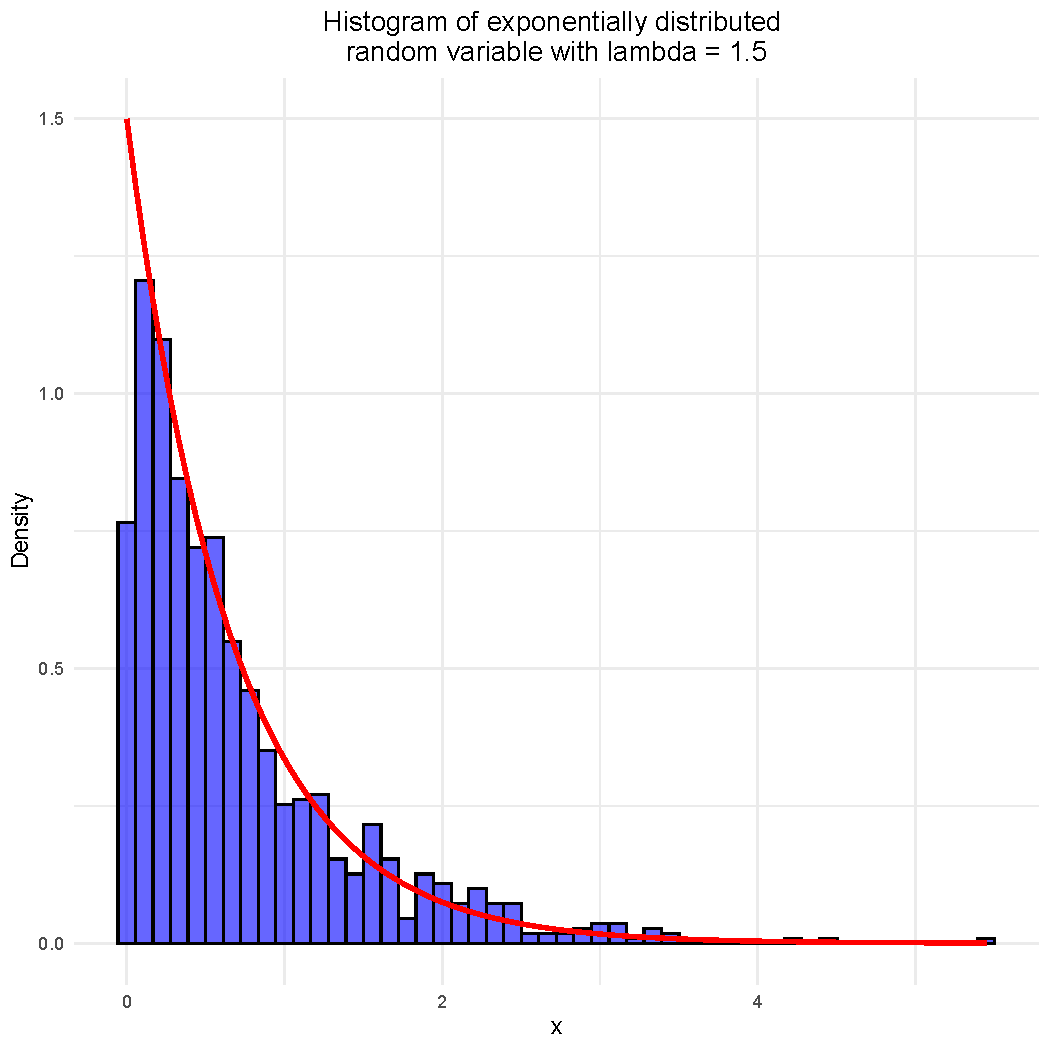
\includegraphics[width=0.7\linewidth]{img/img-1-5-1.jpeg}
	\caption{Exponential distributed random variable; histogram of 1000 generated points and theoretical distribution}
	\label{fig:img-1-6-1}
\end{figure}

\subsubsection{Write down the log-likelihood function for this exponentially distributed random variable.}

For sample $\mathbf{x} = ( x_1, \dots, x_n )^T$ obtained on an exponential distributed random variable $X$, with parameter vector $\mathbf{\theta}=(\lambda)$, the likelihood


\begin{flalign*}
	L(\mathbf{x}, \mathbf{\theta})	&= \prod_{i=1}^{n} f(x_i, \mathbf{\theta}) \\
		&=  \prod_{i=1}^{n} \lambda e^{-\lambda x_i} \\
		&= \lambda^n e^{\sum_{i=1}^n \lambda x_i}
\end{flalign*}

\noindent The log-likelihood is then

$$	
l(\mathbf{x}, \mathbf{\theta}) = n \space log(\lambda) - \lambda \sum_{i=0}^{n} x_i	
$$

\noindent Taking the derivative with respect to $\lambda$,

$$
\frac{\partial l(\mathbf{x}, \mathbf{\theta}) }{\partial\lambda} =
\frac{n}{\lambda} - \sum_{i=0}^{n} x_i	
$$

\noindent for maximum $\frac{\partial l(\mathbf{x}, \mathbf{\theta}) }{\partial\lambda}$

\begin{flalign*}
	L\frac{\partial l(\mathbf{x}, \mathbf{\theta}) }{\partial\lambda}	&= 0 \\ 
	\frac{n}{\lambda} - \sum_{i=0}^{n} x_i	 &= 0 \\
	\frac{n}{\lambda}  &= \sum_{i=0}^{n} x_i	
\end{flalign*}

\noindent So that

\begin{equation}
	\hat{\lambda} = \frac{n}{\sum_{i=0}^{n} x_i	} = \frac{1}{\overline{x}}
\end{equation}


\subsubsection{Evaluate the log-likelihood function for the generated data as a function of $\lambda$, and plot the resulting log-likelihood function against different values of $\lambda$. Present the plot together with the answers.}


The follwoing listing calculates and plots the log-likelihood values for an exponential distribution with varying $\lambda$ values. The resulting plot can be examined in Figure \ref{fig:img-1-6-2}


\begin{lstlisting}
lambda_values <- seq(0.1, 5, by = 0.01)
log_likelihood_values <- sapply(lambda_values,
function(lambda) LL_exponential(lambda, x))

df <- data.frame(lambda_values, log_likelihood_values)

p <- ggplot(df, 
	aes(x = lambda_values, 
	y = log_likelihood_values)) +
geom_point(
	color = "blue",
	alpha = 0.6) +
	labs(
	title = "Log-Likelihood with varying
 lambda values",
	x = "Lambda",
	y = "Log-Likelihood") +
theme_bw()

quartz()
print(p)
\end{lstlisting}

\begin{figure}[H]
	\centering
	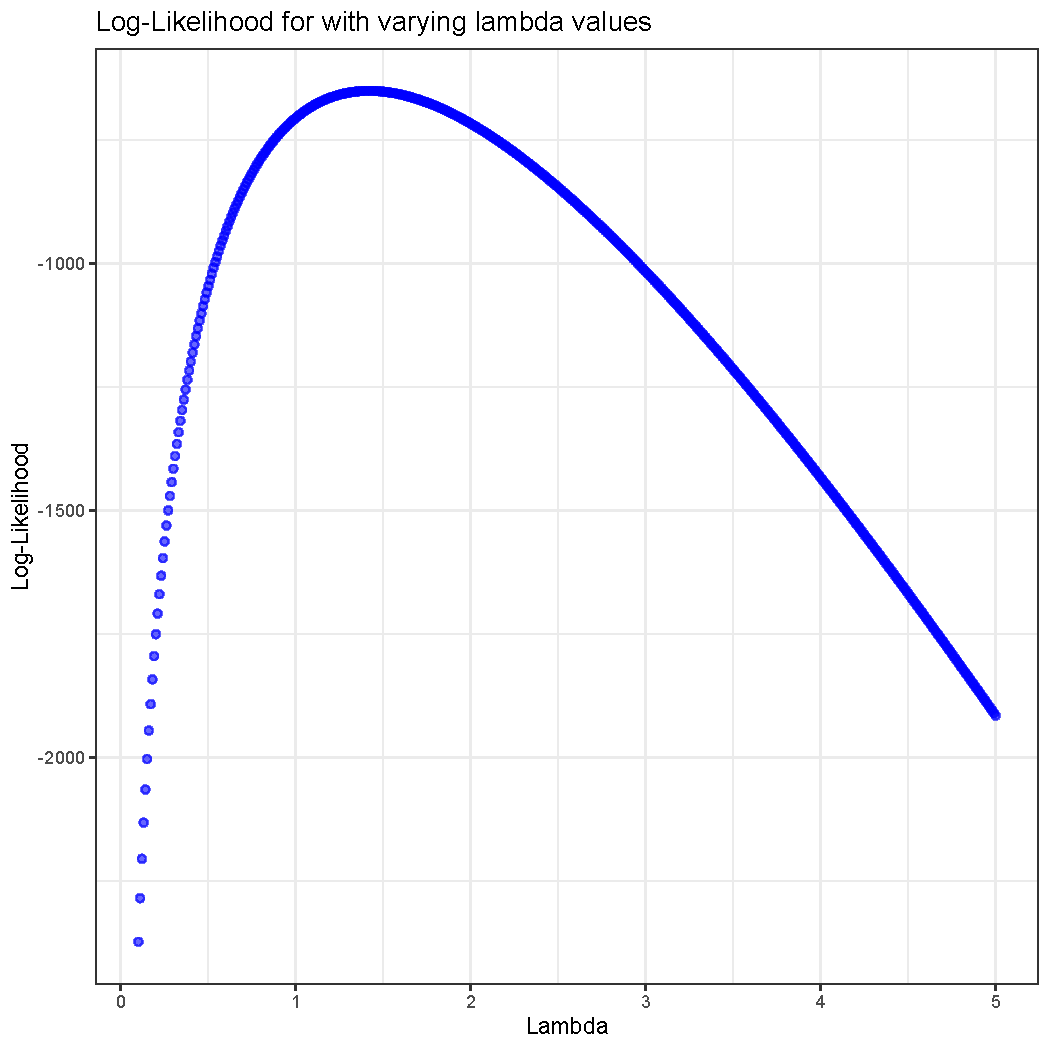
\includegraphics[width=0.7\linewidth]{img/img-1-6-2.jpeg}
	\caption{Log-likelihood plot for an exponential distribution with varying $\lambda$}
	\label{fig:img-1-6-2}
\end{figure}


\subsubsection{Using the plot or otherwise, which estimate for $\lambda$ is the MLE? Give a reason for your answer.}

As we have seen in the previous question, the maximum likelihood estimation is the value for which the derivative of the log-likelihood with respect to lambda is zero, that is the peak of the curve shown in Figure \ref*{fig:img-1-6-2}. This can be easily calculated using the code below. The value obtained for $\hat{\lambda}$ was \textbf{1.43}.

\begin{lstlisting}
max_ll <- max(log_likelihood_values)
max_lambda <- lambda_values[log_likelihood_values == max_ll]
print(glue("Lambda value for maximum log-likelihood is {max_lambda}"))
\end{lstlisting}



\section{title}

\section{title}

\section{Question 4 - Jackknife and bootstrap}

\textbf{Consider 50 observations of bivariate pair $(X,Y)$ in resampling.xlsx. Use the nls command in R to estimate the nonlinear regression $Y=\frac{aX}{b+X} + \epsilon$.}

\bigskip

The code in Listing \ref{lst:nls} performs nonlinear regression on the dataset. The resulting plots are presented in Figure \ref{fig:img-4-1}. The estimated parameters are $\hat{a} = 14.56$ and $\hat{b} = 7.10$.


\begin{figure}[H]
	\captionsetup{type=lstlisting}
	\begin{lstlisting}
library(openxlsx)
library(ggplot2)

# load file
script_dir <- getwd()
file_path <- file.path(script_dir, "resampling.xlsx")
df <- read.xlsx(file_path, colNames = TRUE)

print(c("number of rows: ", nrow(df)))

# estimate the parameters of the model
init_a <- 1
init_b <- 1

nls_model <- nls(y ~ (a * x) / (b + x),
data = df,
start = list(a = init_a, b = init_b))


estimated_params <- coef(nls_model)
a_hat <- estimated_params["a"]
b_hat <- estimated_params["b"]
cat("Estimated a:", a_hat, "\n")
cat("Estimated b:", b_hat, "\n")

# predict the values of y
df$Predicted <- predict(nls_model)
print(head(df))

# plot the data
p <- ggplot(df, aes(x = x  , y = y)) +
geom_point(color = "blue", alpha = 0.5) +
geom_line(aes(
	y = Predicted),
	color = "red",
	linewidth = 1) +
labs(title = "Nonlinear Regression: Y = (aX) / (b+X)",
x = "X", y = "Y") +
theme_minimal()

print(p)
	\end{lstlisting}
\caption{Non linear regression code in R}
\label{lst:nls}
\end{figure}

\begin{figure}[H]
	\centering
	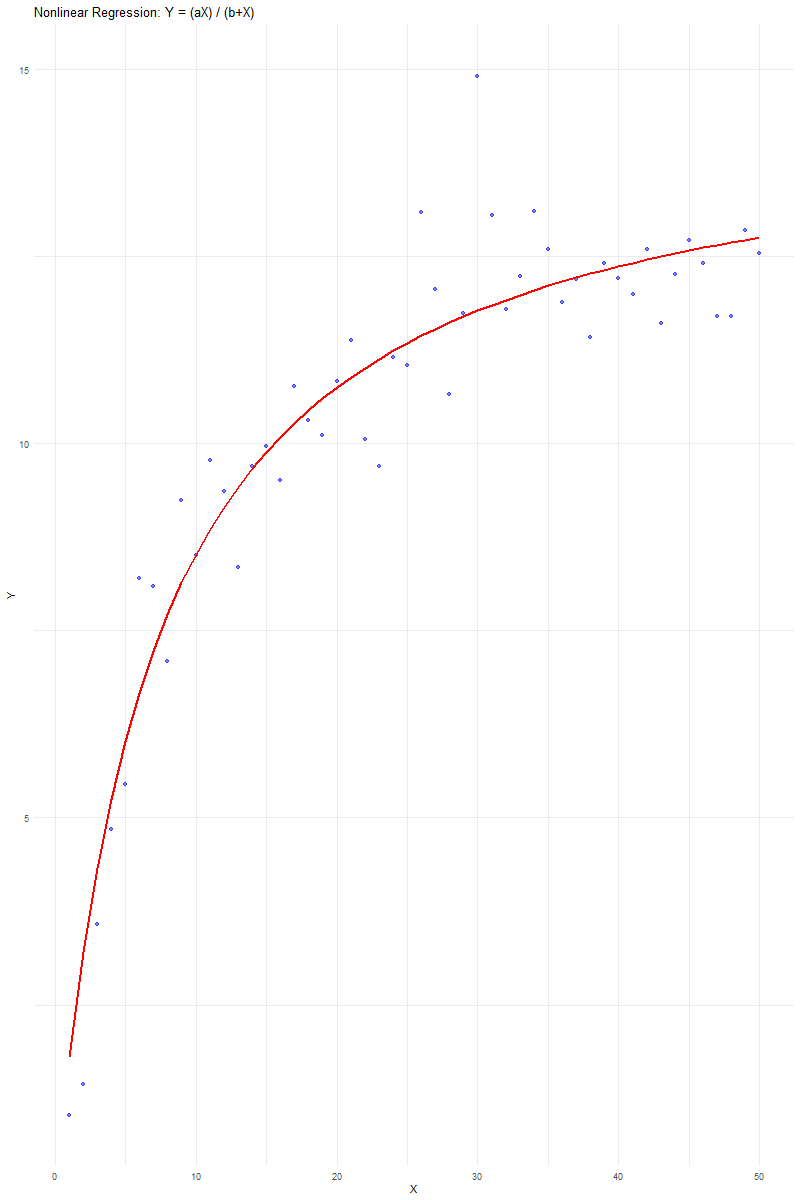
\includegraphics[width=0.7\linewidth]{img/img-4-1}
	\caption{Nonlinear regression fit: observed vs. predicted values}
	\label{fig:img-4-1}
\end{figure}


\subsection{Construct a computer code in R to find the Jackknife and Bootstrap estimators of $a$ and $b$. In the 
	case of Jackknife, section randomly the sampling into 5 partitions of size 10. In the case of 
	Bootstrap, generate 1000 samples of size 100 with replacement. }



The code in Listing \ref{lst:jk} executes the following steps on the data to implement Jackknife resampling with non linear regression. The resulting plots are presented in Figure \ref{fig:img-4-1-1}. The estimated parameters are $\hat{a}_{jk} = 14.504$ and $\hat{b}_{jk} = 6.996$. The code executes the following steps to estimate the parameters:

\begin{enumerate}
	\item \textbf{Shuffle the dataset:} We randomly shuffle the data to remove any ordering bias:

	\item \textbf{Divide the data into $m$ Jackknife partitions:} We split the dataset into $m = 5$ partitions, each missing a unique subset of 5 elements.
	
	\item \textbf{Fit the NLS model for each Jackknife sample:} We fit a nonlinear regression model to each Jackknife sample using Nonlinear Least Squares (NLS) to estimate parameters $a$ and $b$. The model is defined as:
	\begin{equation}
		Y = \frac{aX}{b+X}
	\end{equation}
	and is refitted for each sample $S_{-a}$, which excludes partition $P_a$.
	
	\item \textbf{Compute Jackknife bias-corrected estimates:} The Jackknife estimate for each parameter is calculated using the bias correction formula:
	\begin{equation}
		\hat{\theta}_{\text{jack}} = m \hat{\theta} - (m-1) \hat{\theta}_{(-a)}
	\end{equation}
	where:
	\begin{itemize}
		\item $m = 5$ is the number of partitions.
		\item $\hat{\theta}$ is the parameter estimate from the full dataset.
		\item $\hat{\theta}_{(-a)}$ is the parameter estimate from the jackknife sample with partition $a$ removed.
	\end{itemize}
	
	\item \textbf{Compute final Jackknife estimates for $a$ and $b$:} The final Jackknife estimates for $a$ and $b$ are obtained by averaging the bias-corrected values across all jackknife samples:
	\begin{equation}
		\hat{a}_{jk} = \frac{1}{m} \sum_{a=1}^{m} \hat{a}_{\text{jack}, a}, \quad
		\hat{b}_{jk} = \frac{1}{m} \sum_{a=1}^{m} \hat{b}_{\text{jack}, a}
	\end{equation}
\end{enumerate}



\begin{figure}[H]
	\captionsetup{type=lstlisting}
	\begin{lstlisting}
partition_size <- 5

#shuffle the dataframe
set.seed(123)
df_shuf <- df[sample(nrow(df)), ]

# Generate jackknife samples by removing each fold of 5 elements
# lapply applies a function to each element of a list
# my list is from 1:5
# the function will
# for a = 1 remove element 1 to 5 (5*(1-1)+1):(5*1)
# and so on
# note the - sign -- I am removing the elements
# so the return for each a is y without the elements 1 to 5, 6 to 10, etc.
jackknife_samples <- lapply(1:partition_size,
function(a) df_shuf[-((partition_size * (a - 1) + 1):(partition_size * a)), ])

# we have calculated theta_hat_m before
theta_hat_m <- estimated_params

theta_m_a <- function(data) {
	model <- nls(y ~ (a * x) / (b + x),
	data = data,
	start = list(a = theta_hat_m["a"],
	b = theta_hat_m["b"]))
	return(coef(model)) }

# jackknife estimator for each partition
nlsjk <- sapply(jackknife_samples, function(y_a) partition_size * theta_hat_m - (partition_size - 1) * theta_m_a(y_a))

#evaluating the jackknife estimator of the parametrs
jackknife_estimates <- rowMeans(nlsjk)

a_hat_jk <- jackknife_estimates["a"]
b_hat_jk <- jackknife_estimates["b"]

df$predicted_jk <- (a_hat_jk * df$x) / (b_hat_jk + df$x)

# Plot with Jackknife predictions and legend
p_jk <- ggplot(df, aes(x = x, y = y)) +
geom_point(color = "blue", alpha = 0.5, size = 3) +
geom_line(aes(y = Predicted, color = "Full Sample Prediction"),
linewidth = 1, linetype = "dashed") +
geom_line(aes(y = predicted_jk, color = "Jackknife Prediction"),
linewidth = 1) +
labs(title = "Nonlinear Regression: Full Sample vs. Jackknife",
x = "X", y = "Y", color = "Legend") +
theme_minimal() +
scale_color_manual(values = c("Full Sample Prediction" = "red",
"Jackknife Prediction" = "green"))
	\end{lstlisting}
	\caption{Jackknife resampling code in R}
	\label{lst:jk}
\end{figure}

The resulting plot is shown below in Figure \ref{fig:img-4-1-1}


\begin{figure}[H]
	\centering
	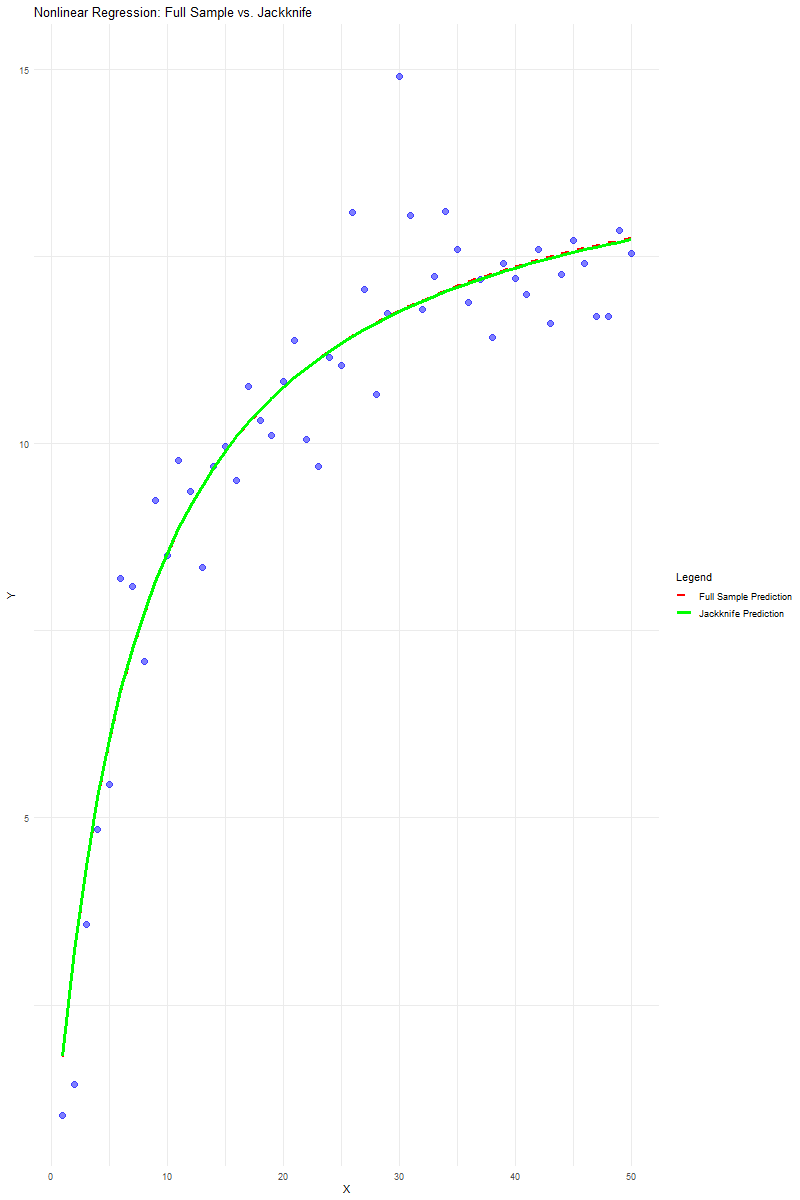
\includegraphics[width=0.7\linewidth]{img/img-4-1-1}
	\caption{Nonlinear regression fit: observed vs. predicted values including Jackknife predictions}
	\label{fig:img-4-1-1}
\end{figure}


The code in Listing \ref{lst:bs} executes the following steps on the data to implement Bootstrap resampling with non linear regression. The resulting plots are presented in Figure \ref{fig:img-4-1-2}. The estimated parameters are $\hat{a}_{bs} = 14.566$ and $\hat{b}_{bs} = 7.110$. The code executes the following steps to estimate the parameters:

\begin{itemize}
	\item \textbf{Generate Bootstrap Samples:}  
	WE create 1000 resampled datasets of size 100 by drawing with replacement from the 50 original observations.
	
	\item \textbf{Fit a Nonlinear Regression Model:}  
	For each bootstrap sample, we estimate parameters $a$ and $b$ using Nonlinear Least Squares (NLS) with the model.
	
	\item \textbf{Compute Bootstrap Estimates:}  
	The final bootstrap estimates are obtained by averaging the parameter estimates from all bootstrap samples:

	\item \textbf{Predict Values Using Bootstrap Estimates:}  
	Using the estimated parameters $\hat{a}_{\text{bs}}, \hat{b}_{\text{bs}}$, we compute the predicted values:
	\begin{equation}
		\hat{y}_{\text{bs}} = \frac{\hat{a}_{\text{bs}} x}{\hat{b}_{\text{bs}} + x}
	\end{equation}
	
\end{itemize}


\begin{figure}[H]
	\captionsetup{type=lstlisting}
	\begin{lstlisting}
num_samples <- 1000
sample_size <- 100

# 1000 bootstrap samples of size 100 with replacement
bootstrap_samples <- lapply(1:num_samples, function(i) df[sample(nrow(df), sample_size, replace = TRUE), ])

fit_bootstrap_nls <- function(data) {
	model <- nls(y ~ (a * x) / (b + x),
	data = data,
	start = list(a = 1, b = 1))  # Initial guesses
	return(coef(model))
}

# Apply NLS to each bootstrap sample
nlsbs <- lapply(bootstrap_samples, fit_bootstrap_nls)

# Convert list of bootstrap estimates to a matrix
bootstrap_estimates <- do.call(rbind, nlsbs)
colnames(bootstrap_estimates) <- c("a", "b")

# Compute mean estimates for a and b
a_hat_bs <- mean(bootstrap_estimates[, "a"], na.rm = TRUE)
b_hat_bs <- mean(bootstrap_estimates[, "b"], na.rm = TRUE)

# Print results
cat("Bootstrap Estimated a:", a_hat_bs, "\n")
cat("Bootstrap Estimated b:", b_hat_bs, "\n")


df$predicted_bs <- (a_hat_bs * df$x) / (b_hat_bs + df$x)


# Plot with Jackknife predictions and legend
p_bs <- ggplot(df, aes(x = x, y = y)) +
geom_point(color = "blue", alpha = 0.5, size = 3) +
geom_line(aes(y = Predicted, color = "Full Sample Prediction"),
linewidth = 1, linetype = "dashed") +
geom_line(aes(y = predicted_jk, color = "Jackknife Prediction"),
linewidth = 1) +
geom_line(aes(y = predicted_bs, color = "Bootstrap Prediction"),
linewidth = 1) +
labs(title = "Nonlinear Regression: Full Sample vs. Jackknife vs. Bootstrap",
x = "X", y = "Y", color = "Legend") +
theme_minimal() +
scale_color_manual(values = c("Full Sample Prediction" = "red",
"Jackknife Prediction" = "green",
"Bootstrap Prediction" = "blue"))
	\end{lstlisting}
	\caption{Bootstrap resampling code in R}
	\label{lst:bs}
\end{figure}


\begin{figure}[H]
	\centering
	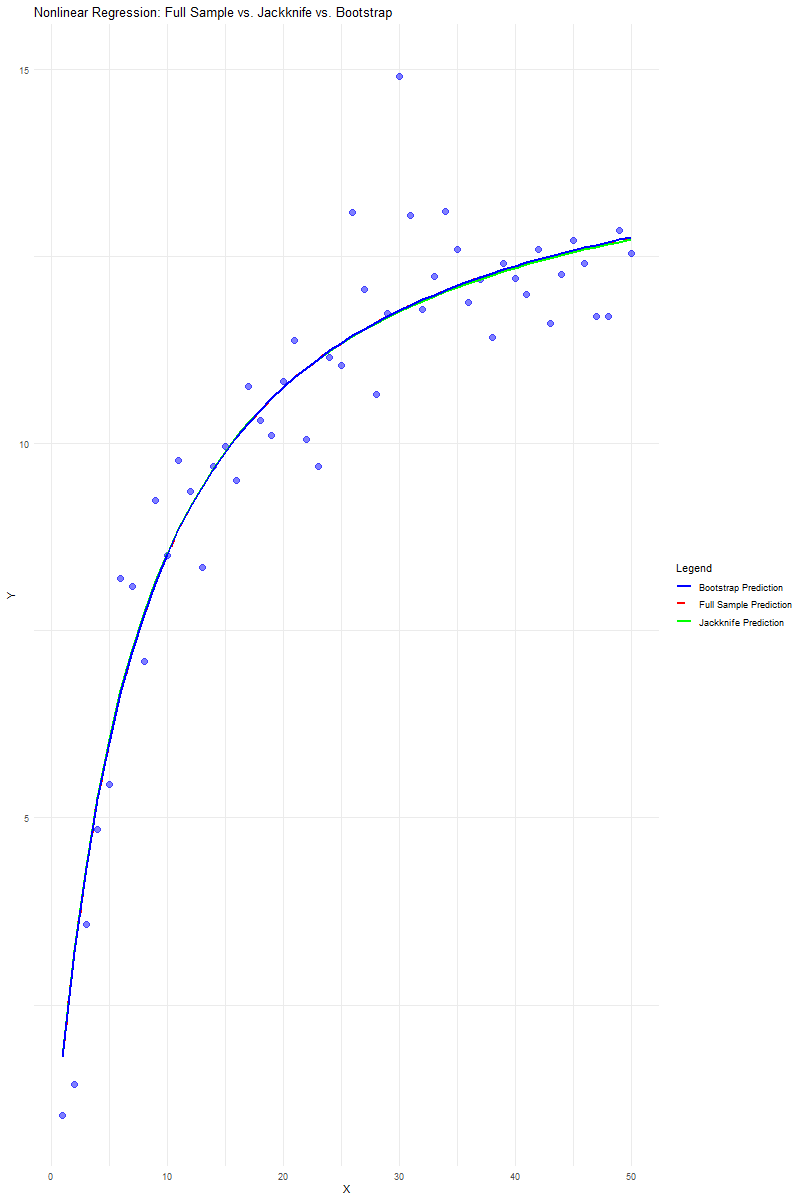
\includegraphics[width=0.7\linewidth]{img/img-4-1-2}
	\caption{Nonlinear regression fit: observed vs. predicted values including Jackknife and Bootstrap predictions}
	\label{fig:img-4-1-2}
\end{figure}

\subsection{For the Jackknife estimator, find a 95\% confidence interval using the normal distribution and the t-distribution. For the Bootstrap estimator, find a 95\% normal, t and empirical confidence intervals.}

%To estimate the uncertainty in our parameter estimates, we compute 95\% confidence intervals using the following:
%
%\begin{enumerate}
%	\item \textbf{Compute the standard error (SE):}  
%	\begin{equation}
%		SE = \sqrt{\frac{c}{n} \sum_{i=1}^{n} (\hat{\theta}_{i} - \hat{\theta})^2}
%	\end{equation}
%	where:
%	\begin{itemize}
%		\item $\hat{\theta}_{i}$ is the estimate from the $i$-th resample.
%		\item $\hat{\theta}$ is the mean of all estimates.
%		\item $n$ is the number of resamples: 
%		\begin{itemize}
%			\item number of partitions for Jackknife
%			\item number of resamples for Bootstrap
%		\end{itemize}
%		\item $c$ is a correction factor:
%		\begin{itemize}
%			\item For Jackknife: $c = (m-1)/m$ as bias correction is necessary
%			\item For Bootstrap: $c = 1$  as no correction needed
%		\end{itemize}
%	\end{itemize}
%	
%	\item \textbf{Compute the 95\% confidence interval using the Normal Distribution:}
%	\begin{equation}
%		CI_{\text{normal}} = \hat{\theta} \pm Z_{0.975} \cdot SE
%	\end{equation}
%	where $Z_{0.975} = 1.96$ for a 95\% confidence level.
%	
%	\item \textbf{Compute the 95\% confidence interval using the t-distribution:}
%	\begin{equation}
%		CI_{\text{t}} = \hat{\theta} \pm t_{0.975, df} \cdot SE
%	\end{equation}
%	where:
%	\begin{itemize}
%		\item For Jackknife: $df = m - 1$
%		\item For Bootstrap: $df = B - 1$
%	\end{itemize}
%	
%	\item \textbf{Compute the 95\% confidence interval using the Empirical (Percentile) Method (Bootstrap only):}
%	\begin{equation}
%		CI_{\text{empirical}} = \left[ Q_{0.025}, Q_{0.975} \right]
%	\end{equation}
%	where $Q_{0.025}$ and $Q_{0.975}$ are the 2.5th and 97.5th percentiles of the bootstrap estimates.
%\end{enumerate}
%
%\bigskip

\noindent The following results were obtained for the Jackknife resampling method:

\begin{itemize}
	\item 95\% conf. interval for a using normal distribution: [ 14.14397 , 14.86412 ]
	\item 95\% conf. interval for b using normal distribution: [ 6.356596 , 7.635241 ]
	\item 95\% conf. interval for a using t-distribution: [ 13.99397 , 15.01412 ]
	\item 95\% conf. interval for b using t-distribution: [ 6.090267 , 7.90157 ]
\end{itemize}


\noindent The following results were obtained for the Bootstrap resampling method:

\begin{itemize}
	\item conf. interval for a using normal distribution: [ 14.07722 , 15.05515 ]
	\item conf. interval for b using normal distribution: [ 6.111358 , 8.109172 ]
	\item conf. interval for a using t-distribution: [ 14.07663 , 15.05575 ]
	\item conf. interval for b using t-distribution: [ 6.110146 , 8.110384 ]
	\item conf. interval for a using empirical distribution: [ 14.08458 , 15.08578 ]
	\item conf. interval for b using empirical distribution: [ 6.132766 , 8.113393 ]
\end{itemize}

\begin{table}[h]
	\centering
	\begin{tabular}{|c|c|c|}
		\hline
		\textbf{Method} & \textbf{Confidence Interval for $a$} & \textbf{Confidence Interval for $b$} \\
		\hline
		\multicolumn{3}{|c|}{\textbf{Jackknife Resampling}} \\
		\hline
		Normal Distribution & [14.14397, 14.86412] & [6.356596, 7.635241] \\
		t-Distribution & [13.99397, 15.01412] & [6.090267, 7.90157] \\
		\hline
		\multicolumn{3}{|c|}{\textbf{Bootstrap Resampling}} \\
		\hline
		Normal Distribution & [14.07722, 15.05515] & [6.111358, 8.109172] \\
		t-Distribution & [14.07663, 15.05575] & [6.110146, 8.110384] \\
		Empirical Distribution & [14.08458, 15.08578] & [6.132766, 8.113393] \\
		\hline
	\end{tabular}
	\caption{Confidence Intervals for Parameters $a$ and $b$ Using Jackknife and Bootstrap Methods}
	\label{tab:ci_results}
\end{table}


\section{Question 5 – The EM Algorithm }

Consider a univariate $K$-Gaussian mixture model with probability density function:

$$
f(x) = \sum_{l=1}^{K} \pi_l \phi(x, \mu_l, \sigma_l)
$$

\noindent such that $\sum_{l=1}^{K} \pi_l = 1$ and $\pi_l > 0$ for all $l$, and where $\phi(x, \mu, \sigma)$ is the Gaussian density function. The EM algorithm for this works as follows:

\begin{enumerate}
	\item Initialise $\mu_1^{(0)}, \dots, \mu_K^{(0)}, \sigma_1^{(0)}, \dots, \sigma_K^{(0)}, \pi_1^{(0)}, \dots, \pi_K^{(0)}$.
	
	\item Let 
	$$
	\gamma_n^{(j,k)} = \frac{\pi_k \phi(x_n | \mu_k^{(j-1)}, \sigma_k^{(j-1)})}{\sum_{i=1}^{K} \pi_i \phi(x_n | \mu_i^{(j-1)}, \sigma_i^{(j-1)})}.
	$$
	
	\item Let
	$$
	\mu_k^{(J)} = \frac{1}{N_k} \sum_{n=1}^{N} \gamma_n^{(j,k)} x_n, 
	$$
	$$
	\sigma_k^{(J)} = \sqrt{\frac{1}{N_k} \sum_{n=1}^{N} \gamma_n^{(j,k)} (x_n - \mu_k^{(J)})^2},
	$$
	and 
	$$
	\pi_k^{(J)} = \frac{N_{jk}}{N},
	$$
	where
	$$
	N_{jk} = \sum_{n=1}^{N} \gamma_n^{(j,k)}.
	$$
\end{enumerate}

\subsection{Simulate 1000 readings from a mixture Gaussian distribution with 3 or more Gaussians.}

The following function generalizes the code provided in the question so that an arbitrary number of samples are generated from any number of Gaussian distributions. The function also lists the number of samples selected from each Gaussian to ensure that acceptable proportions were attained for each sample and plots a distribution of the data and plots of the Gaussians.

\begin{figure}[H]
	\captionsetup{type=lstlisting}
	\begin{lstlisting}
library(ggplot2)

generate_samples <- function(
mixing_coefficients,
means,
standard_deviations,
number_of_samples = 1000) {
	
	# should check that lengths are equal
	
	data <- c()
	choices_count <- rep(0, length(mixing_coefficients))
	
	# select one of the gaussian distributions according
	# to the mixing coefficients
	choices <- sample(
	x = seq_along(mixing_coefficients),
	size = number_of_samples,
	prob = mixing_coefficients,
	replace = TRUE)
	
	# let us see that the number of selections make sense
	for (i in 1:number_of_samples){
		choices_count[choices[i]] <- choices_count[choices[i]] + 1
	}
	print(choices_count)
	
	# for each selection, sample from the gaussian
	data <- c(
	data,
	rnorm(
	n = number_of_samples,
	mean = means[choices],
	sd = standard_deviations[choices]))
	
	# plot histogram and gaussian curves
	df <- data.frame(data)
	
	p <- ggplot(df, aes(x = data)) +
	geom_histogram(
	aes(y = ..density..),
	bins = 30,
	fill = "blue",
	alpha = 0.6) +
	stat_function(fun = function(x) {
		Reduce(`+`, lapply(1:length(means), function(i) {
			dnorm(
			x = x,
			mean = means[i],
			sd = standard_deviations[i]) * mixing_coefficients[i]
		}))
	}, color = "red") +
	labs(title = "Histogram of Mixture of Gaussians",
	x = "Value",
	y = "Density") +
	theme_bw()
	
	print(p)
}
	\end{lstlisting}
	\caption{Gaussian mixture sample generation code in R}
	\label{lst:gausmix}
\end{figure}

\noindent Data from the mixed Gaussian distributions was subsequently generated using the parameters below. The plot that was obtained as a result of this process is shown in Figure \ref{fig:img-5-1}

\begin{table}[h]
	\centering
	\renewcommand{\arraystretch}{1.2} % Adjust row height
	\begin{tabular}{|c|c|c|}
		\hline
		$\pi_1 = 0.2$ & $\mu_1 = 6$  & $\sigma_1 = 2.0$  \\
		\hline
		$\pi_2 = 0.5$ & $\mu_2 = 0$  & $\sigma_2 = 1.0$  \\
		\hline
		$\pi_3 = 0.3$ & $\mu_3 = -7$ & $\sigma_3 = 1.5$  \\
		\hline
	\end{tabular}
\end{table}

\begin{figure}[H]
	\captionsetup{type=lstlisting}
	\begin{lstlisting}
mixing_coefficients <- c(0.2, 0.5, 0.3)
means <- c(6, 0, -7)
standard_deviations <- c(2, 1, 1.5)

generate_samples(mixing_coefficients, means, standard_deviations)			
		\end{lstlisting}
	\caption{Generation of data for this question}
	\label{lst:gem-gausmix}
\end{figure}

\begin{figure}[H]
	\centering
	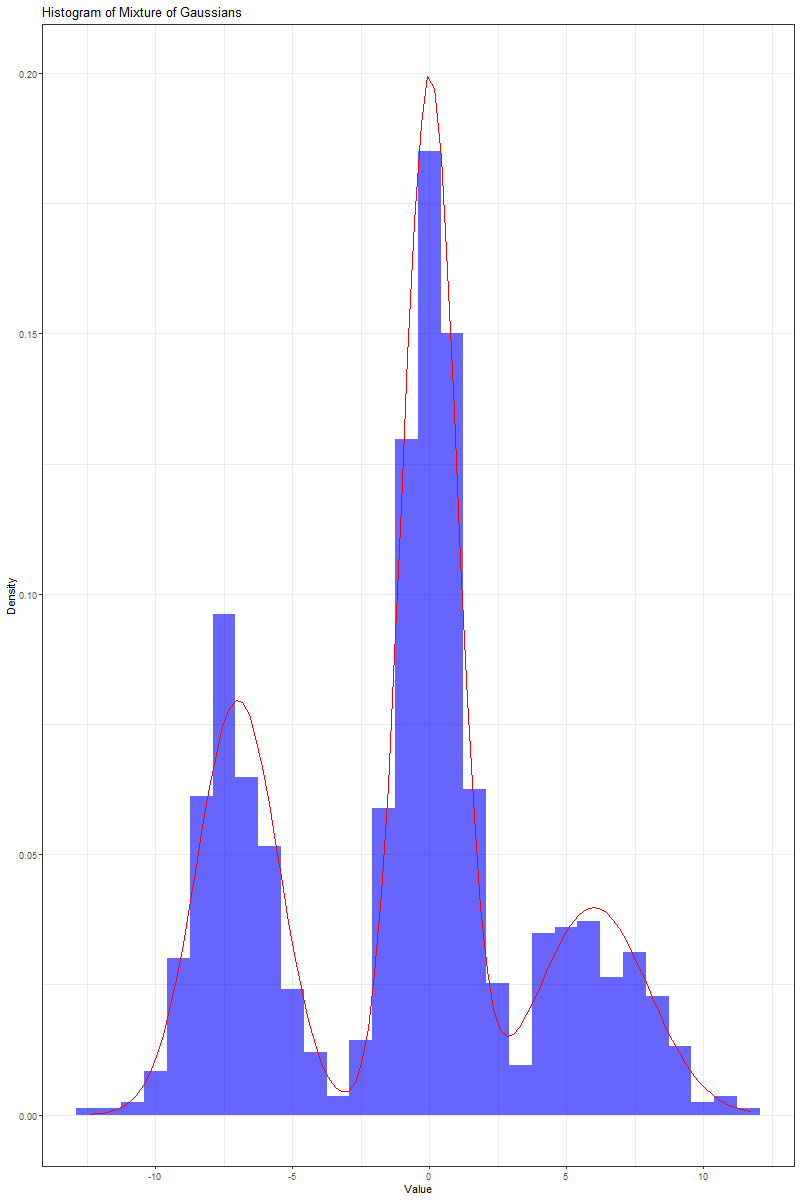
\includegraphics[width=0.5\linewidth]{img/img-5-1}
	\caption{Distribution of generated data}
	\label{fig:img-5-1}
\end{figure}


\subsection{Determine initial values $\mu_1^{(0)}, \dots, \mu_K^{(0)}, \sigma_1^{(0)}, \dots, \sigma_K^{(0)}, \pi_1^{(0)}, \dots, \pi_K^{(0)}$ 	using a K-means clustering approach or otherwise.
}

The function in Listing \ref{lst:kmeans} is a custom implementation of a k-means algorithm to initialize parameters($\mu^{(0)}$, $\sigma^{(0)}$, and $\pi^{(0)}$) for a Gaussian mixture model. Its salient features are the following:
\begin{itemize}
	\item After the initial centroids are randomly selected, the k-means algorithm iteratively assigns the data point to the closest centroid based on the absolute distance. The cluster centroids are then updated as the means of the points assigned to each cluster until the change in centroids is small or the threshold number of iterations is reached.
	\item The means of each centroid is, as we have discussed above, the centroid of each cluster.
	\item the standard deviation is calculated as follows
	$$
	\sigma_j =
	\begin{cases}
		\sqrt{\frac{1}{n_j} \sum_{x_i \in C_j} (x_i - \mu_j)^2}, & \text{if } n_j > 0 \\
		0, & \text{otherwise}
	\end{cases}
	$$
	Where:
	\begin{itemize}
		\item $\sigma_j$ is the standard deviation for cluster $j$,
		\item $C_j$ is the set of points in cluster $j$,
		\item $n_j$ is the number of points in cluster $j$,
		\item $x_i$ are the individual data points in cluster $j$,
		\item $\mu_j$ is the centroid (mean) of cluster $j$,
	\end{itemize}
	
	\item The initial values for the mixing coefficients of the Gaussian Mixture Model are computed as:
	
	$$
	\pi_j =
	\begin{cases}
		\frac{n_j}{N}, & \text{if } n_j > 0 \\
		0, & \text{otherwise}
	\end{cases}
	$$
	
	Where:
	\begin{itemize}
		\item $\pi_j$ is the mixing coefficient for cluster $j$,
		\item $n_j$ is the number of data points in cluster $j$,
		\item $N$ is the total number of data points in the dataset,
	\end{itemize}
	
\end{itemize}


\begin{figure}[H]
	\captionsetup{type=lstlisting}
	\begin{lstlisting}
initial_values_knn <- function(data, k = 3) {
	set.seed(42)  # For reproducibility
	
	# Randomly select k initial centroids
	centroids <- sample(x = data, size = k, replace = FALSE)
	
	# Initialize empty clusters
	clusters <- vector(mode = "list", length = k)
	
	for (iteration in 1:100) {
		# Reset clusters
		clusters <- vector(mode = "list", length = k)
		
		# Assign each data point to the closest centroid
		for (item in data) {
			distances <- abs(item - centroids)
			closest_centroid <- which.min(distances)
			clusters[[closest_centroid]] <- c(clusters[[closest_centroid]], item)
		}
		
		# Compute new centroids
		new_centroids <- sapply(1:k, function(i) {
			if (length(clusters[[i]]) > 0) {
				mean(clusters[[i]])
			} else {
				centroids[i]  # Keep old centroid if no points are assigned
			}
		})
		
		# Check for convergence
		if (max(abs(new_centroids - centroids)) < 0.0001) {
			break
		}
		
		centroids <- new_centroids
	}
	
	# Compute standard deviations
	clusters_standard_devs <- sapply(1:k, function(cluster_idx) {
		if (length(clusters[[cluster_idx]]) > 0) {
			sqrt(sum((clusters[[cluster_idx]] - centroids[cluster_idx])^2) / length(clusters[[cluster_idx]]))
		} else {
			0
		}
	})
	
	# Compute mixing coefficients for each cluster
	mixing_coefficients <- sapply(1:k, function(cluster_idx) {
		length(clusters[[cluster_idx]]) / length(data)
	})
	
	return(list(
	centroids = centroids,
	standard_devs = clusters_standard_devs,
	mixing_coefficients = mixing_coefficients))
}
		
		\end{lstlisting}
	\caption{k-means algorithm to compute the initial values of the mixed Gaussian model parameters}
	\label{lst:kmeans}
\end{figure}

The results obtained from this function are as follows:

\bigskip

\begin{table}[h]
	\centering
	\renewcommand{\arraystretch}{1.2} % Adjust row height
	\begin{tabular}{|c|c|c|}
		\hline
		$\pi_1 = 0.179$ & $\mu_1 = 6.353$  & $\sigma_1 = 1.685$  \\
		\hline
		$\pi_2 = 0.545$ & $\mu_2 = 0.104$  & $\sigma_2 = 1.107$  \\
		\hline
		$\pi_3 = 0.276$ & $\mu_3 = -6.942$ & $\sigma_3 = 1.508$  \\
		\hline
	\end{tabular}
	\caption{Estimated parameters for the initial values of Gaussian mixture model}
	\label{tab:gmm_parameters}
\end{table}

\subsection{Run the EM algorithm for a number of iterations. Print 
	$\mu_1^{(j)}, \dots, \mu_k^{(j)}, \sigma_1^{(j)}, \dots, \sigma_k^{(j)}, \pi_1^{(j)}, \dots, \pi_k^{(j)}$ 
	for each iteration, and also the log-likelihood, which is given by:
	$
	\sum_{n=1}^{N} \ln \left( \sum_{l=1}^{K} \phi(x_i | \mu_l^{(j)}, \sigma_l^{(j)}) \right).
	$
	Determine when to stop the EM algorithm, either via a maximum number of iterations or through a convergence criterion. However, ensure that the EM algorithm has converged. Plot the trajectory of the estimates and the likelihood by iteration to illustrate this.
}



\begin{figure}[H]
	\captionsetup{type=lstlisting}
	\begin{lstlisting}
expectation_step <- function(data, means, standard_deviations, mixing_coefficients) {
	
	number_of_gaussians <- length(mixing_coefficients)
	
	# Initialize gamma matrix
	gamma <- matrix(0, nrow = length(data), ncol = number_of_gaussians)
	
	# Calculate denominator (total probability for each data point)
	den_total <- 0
	for (k in 1:number_of_gaussians) {
		den_total <- den_total + mixing_coefficients[k] * dnorm(data, mean = means[k], sd = standard_deviations[k])
	}
	
	# Calculate numerator and compute gamma
	for (k in 1:number_of_gaussians) {
		gamma[, k] <- (mixing_coefficients[k] * dnorm(data, mean = means[k], sd = standard_deviations[k])) / den_total
	}
	
	return(gamma)
}			
		\end{lstlisting}
	\caption{Estimation step code in R}
	\label{lst:em-est}
\end{figure}


\begin{figure}[H]
	\captionsetup{type=lstlisting}
	\begin{lstlisting}

maximization_step <- function(data, gamma, means, standard_deviations, mixing_coefficients) {
	
	no_gaussians <- length(mixing_coefficients)
	m <- length(data)
	
	# Compute cluster responsibilities
	m_c <- colSums(gamma)  # Sum of responsibilities for each Gaussian
	
	# Compute new mixing coefficients
	new_mixing_coefficients <- m_c / m
	
	# Initialize new means and standard deviations
	new_means <- numeric(no_gaussians)
	new_standard_deviations <- numeric(no_gaussians)
	
	# Compute new means and standard deviations for each Gaussian
	for (k in 1:no_gaussians) {
		new_means[k] <- sum(gamma[, k] * data) / m_c[k]
		new_standard_deviations[k] <- sqrt(sum(gamma[, k] * (data - means[k])^2) / m_c[k])
	}
	
	return(list(
	means = new_means,
	standard_devs = new_standard_deviations,
	mixing_coefficients = new_mixing_coefficients
	))
}

	\end{lstlisting}
	\caption{Jackknife resampling code in R}
	\label{lst:jk}
\end{figure}

\begin{figure}[H]
	\captionsetup{type=lstlisting}
	\begin{lstlisting}
			
		\end{lstlisting}
	\caption{Jackknife resampling code in R}
	\label{lst:jk}
\end{figure}

\begin{figure}[H]
	\captionsetup{type=lstlisting}
	\begin{lstlisting}
			
		\end{lstlisting}
	\caption{Jackknife resampling code in R}
	\label{lst:jk}
\end{figure}



\bibliography{references}
\bibliographystyle{plain}

\end{document}

%\begin{figure}[H]
%	\captionsetup{type=lstlisting}
%	\begin{lstlisting}
%		
%	\end{lstlisting}
%	\caption{Jackknife resampling code in R}
%	\label{lst:jk}
%\end{figure}
%
